% Rack technology-cooling-system (TCS) control volume for the synthetic v1.1 suite.
% Drawn at IEEE single-column width (3.5 in); include at \columnwidth without scaling.
% Values shown are the declared synthetic baseline (suite.json), not measurements.
% Build: pdflatex fig_rack_tcs_schematic.tex
\pdfinfoomitdate=1 \pdftrailerid{} \pdfsuppressptexinfo=-1
\documentclass[10pt,border=1pt]{standalone}
\usepackage[helvet]{sfmath}
\usepackage[scaled=1.0]{helvet}
\renewcommand{\familydefault}{\sfdefault}
\usepackage{tikz}
\usetikzlibrary{arrows.meta,calc}

\definecolor{supply}{HTML}{0072B2}
\definecolor{return}{HTML}{D55E00}
\definecolor{air}{HTML}{7F7F7F}
\definecolor{plate}{HTML}{D9D9D9}

\begin{document}
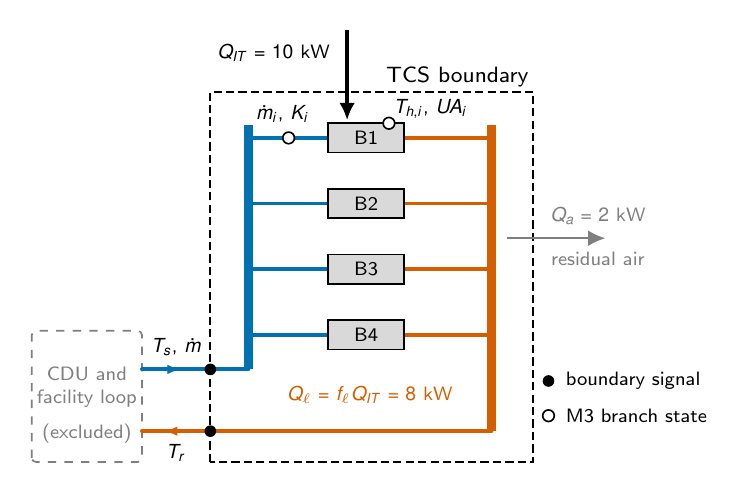
\begin{tikzpicture}[
    x=0.965cm, y=0.98cm,
    font=\scriptsize,
    pipe/.style={line width=1.4pt, line cap=round},
    manifold/.style={line width=3.2pt, line cap=butt},
    obs/.style={circle, fill=black, inner sep=0pt, minimum size=4.2pt},
    hidden/.style={circle, draw=black, fill=white, line width=0.6pt, inner sep=0pt, minimum size=4.2pt},
    heat/.style={-{Latex[length=2.2mm,width=2.0mm]}},
  ]
  % ------------------------------------------------------------------ CDU (outside boundary)
  \draw[air, dashed, line width=0.6pt, rounded corners=1.5pt] (0,0.25) rectangle (1.45,1.95);
  \node[air, align=center] at (0.725,1.22) {CDU and\\facility loop};
  \node[air, align=center] at (0.725,0.62) {(excluded)};

  % ------------------------------------------------------------------ TCS boundary
  \draw[black, dash pattern=on 3pt off 1.5pt, line width=0.7pt] (2.35,0.25) rectangle (6.6,5.05);
  \node[anchor=south east, inner sep=1.5pt] at (6.6,5.05) {\footnotesize TCS boundary};

  % ------------------------------------------------------------------ manifolds
  \draw[manifold, supply] (2.85,1.45) -- (2.85,4.62);
  \draw[manifold, return] (6.05,0.65) -- (6.05,4.62);

  % ------------------------------------------------------------------ supply and return lines
  \draw[pipe, supply] (1.45,1.45) -- (2.85,1.45);
  \draw[pipe, return] (6.05,0.65) -- (1.45,0.65);
  \draw[supply, -{Latex[length=1.6mm]}] (1.6,1.45) -- (1.95,1.45);
  \draw[return, -{Latex[length=1.6mm]}] (2.1,0.65) -- (1.75,0.65);

  % ------------------------------------------------------------------ four parallel branches
  \foreach \y/\name in {4.45/B1, 3.6/B2, 2.75/B3, 1.9/B4} {
    \draw[pipe, supply] (2.85,\y) -- (3.9,\y);
    \draw[pipe, return] (4.9,\y) -- (6.05,\y);
    \draw[fill=plate, draw=black, line width=0.6pt] (3.9,\y-0.19) rectangle (4.9,\y+0.19);
    \node at (4.4,\y) {\name};
  }

  % ------------------------------------------------------------------ heat paths
  \draw[heat, black, line width=1.6pt] (4.15,5.85) -- (4.15,4.68);
  \node[anchor=east] at (4.05,5.55) {$Q_{IT} = 10$ kW};
  \draw[heat, air, line width=0.8pt] (6.25,3.15) -- (7.55,3.15);
  \node[air, anchor=south] at (7.45,3.2) {$Q_a = 2$ kW};
  \node[air, anchor=north] at (7.45,3.1) {residual air};
  \node[return, align=center] at (4.45,1.12) {$Q_\ell = f_\ell Q_{IT} = 8$ kW};

  % ------------------------------------------------------------------ boundary observables
  \node[obs] at (2.35,1.45) {};
  \node[obs] at (2.35,0.65) {};
  \node[anchor=south] at (1.9,1.5) {$T_s$, $\dot m$};
  \node[anchor=north] at (1.9,0.6) {$T_r$};

  % ------------------------------------------------------------------ internal (branch) states
  \node[hidden] at (3.38,4.45) {};
  \node[hidden] at (4.7,4.64) {};
  \node[anchor=south] at (3.3,4.52) {$\dot m_i$, $K_i$};
  \node[anchor=south west, inner sep=1pt] at (4.72,4.66) {$T_{h,i}$, $UA_i$};

  % ------------------------------------------------------------------ key
  \node[obs] at (6.8,1.3) {};
  \node[anchor=west] at (6.9,1.3) {boundary signal};
  \node[hidden] at (6.8,0.85) {};
  \node[anchor=west] at (6.9,0.85) {M3 branch state};
\end{tikzpicture}
\end{document}
